\section{准入与账户体系}\label{sec:hierarchy}

在比特币或者以太坊等其它分布式账本系统中,账户与账户之间的关系是平等的,账户体系是扁平化的,没有层级关系。与此不同,在 Libra 系统中,根据金融监管的需要设计了特定的组织安排,表现在账户体系上,就形成了层次化的账户,不同类型的账户被授予不同的责任和权限。Libra 的账户分为3个类别:

\begin{enumerate}
    \item \textbf{Libra 系统账户}

        系统账户在 Libra 初始化阶段创建,由 Libra 协会负责管理。Libra 系统账户负责系统的版本升级、系统智能合约管理,以及为 Libra 协会成员和合规机构创建账户。
        
    \item \textbf{合规机构账户}

        一个合规机构需要向 Libra 注册,提供法人证明、金融牌照等相关资质证明,审核通过后由 Libra 系统账户创建。

    \item \textbf{企业和个人账户}
    
        所有的企业与个人账户必须向某一个合规机构注册,通过 KYC 审核之后,委托合规机构创建账户。
    
\end{enumerate}

这三种账户形成了一个金字塔结构,下层的账户是由上层的账户创建并且管理的。最上层的 Libra 系统账户可以视为根账户,从它开始派生出其它所有账户。中间的合规机构账户是 Libra 协会根据各个行政辖区的金融监管政策,审核通过的相关机构,负责执行相应的AML/CFT等合规条款。这两种账户都是知名账户,必须公开自己的真实身份,并且接受公众的监督。
最底层的账户是 Libra 用户的,无论是个人还是企业,必须向对应辖区的合规机构实名注册才能创建。企业和个人账户可以选择成为知名账户或者匿名账户。如果是匿名账户,那么由合规机构保护真实身份信息的隐私性,从链上的公开数据是无法识别其真实身份。

\begin{figure}[h!]
    \centering
    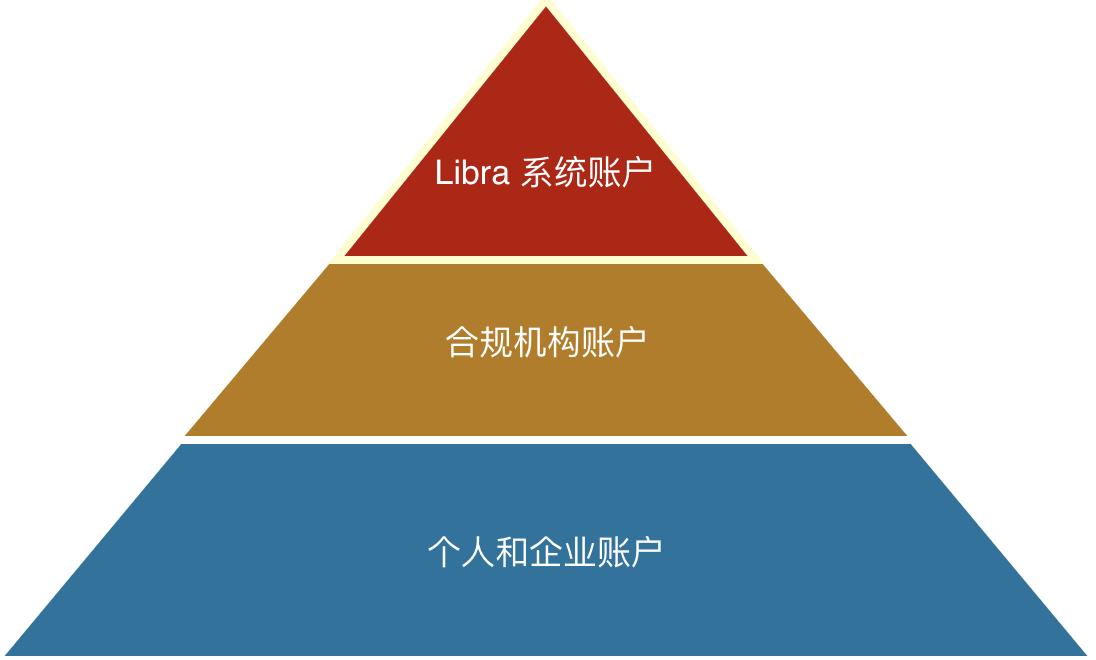
\includegraphics[width=10cm, keepaspectratio]{images/ledger_hierarchy.png}
    \caption{Libra 账户层次结构}
    \label{fig:hierarchy}
\end{figure}
